\documentclass{article}
\usepackage{boxedminipage}
\usepackage{color}
\usepackage{amsmath}
\usepackage{amssymb}
\usepackage{amsthm}
\usepackage{bm}
\usepackage{xy}
\usepackage{geometry}
\usepackage{fullpage}
\usepackage{graphicx}
\usepackage{float}
\usepackage{url}            %for \url{www.---} in bibliography
\DeclareGraphicsExtensions{.png}

\title{The 2D Helmholtz decomposition of a vector field with open boundaries}
\author{Ryan Holmes} \geometry{a4paper}

\begin{document}
\maketitle
\section{The Problem}

Given a velocity field $\bm{u}(x,y) = u(x,y)\bm{\hat{i}} +
v(x,y)\bm{\hat{j}}$ defined on a 2D space, we place a square inside
the field and define this as our boundary $\mathcal{B}$ with zonal
length $L_x$ and meridional length $L_y$. The problem is then to
\textbf{find a $\psi$ and a $\phi$ such that}
\begin{eqnarray}
  \bm{u}(x,y) & = & \nabla\phi + \nabla\psi \times \bm{\hat{k}} \nonumber \\
  \Longrightarrow u(x,y) & = & \frac{\partial\phi}{\partial x} + \frac{\partial\psi}{\partial y} \nonumber \\
  \Longrightarrow v(x,y) & = & \frac{\partial\phi}{\partial y} - \frac{\partial\psi}{\partial x} \nonumber
\end{eqnarray}
within the area $A$ bounded by $\mathcal{B}$. This involves solving
the system of poisson equations
\begin{eqnarray}
\label{Pphi}  \nabla^2\phi & = & \nabla\cdot\bm{u} \\
\label{Ppsi}  \nabla^2\psi & = & -\nabla \times \bm{u} 
\end{eqnarray}
which are coupled through the boundary conditions
\begin{eqnarray}
  \frac{\partial\phi}{\partial x}|_{\mathcal{B}} +
  \frac{\partial\psi}{\partial y}|_{\mathcal{B}} & = & u(x,y)|_{\mathcal{B}}\label{BC1} \\
  \frac{\partial\phi}{\partial y}|_{\mathcal{B}} -
  \frac{\partial\psi}{\partial x}|_{\mathcal{B}} & = & v(x,y)|_{\mathcal{B}}\label{BC2}
\end{eqnarray}
As the potentials $\phi$, $\psi$ are only defined up to a constant, we
set 
\begin{equation} \phi(0,0) = 0 = \psi(0,0) \end{equation}

\noindent Applying the divergence theorem to our boundary $\mathcal{B}$ gives
\begin{equation} 
\int_A \nabla\cdot\bm{u} \,dx dy = \int_\mathcal{B} \bm{u}\cdot\bm{n}\,\,dl
\end{equation}
where $\bm{n}$ is the outward pointing normal and $dl$ is a line
element along the boundary. Substituing in the boundary conditions for
the velocity gives a constraint on the velocity potential $\phi$
\begin{equation}\label{phic}
\int_{\mathcal{B}} \frac{\partial \phi}{\partial n} \,dl = \int_A
\nabla\cdot\bm{u} \,dx dy
\end{equation}
Similarly applying Stokes' theorem to our boundary $\mathcal{B}$
\begin{equation} 
\int_A \nabla\times\bm{u} \,dx dy = -\int_\mathcal{B} \bm{u}\cdot\bm{t}\,dl,
\end{equation}
where $\bm{t}$ is the tangent vector to the boundary, gives a
constraint on the streamfunction $\psi$
\begin{equation}\label{psic}
\int_{\mathcal{B}} \frac{\partial \psi}{\partial n} \,dl = -\int_A
\nabla\times\bm{u} \,dx dy
\end{equation}
These constraints must also be satisfied by the solution.

\section{Continous method description}

The boundary conditions \eqref{BC1} and \eqref{BC2} are applied only
to the velocity and thus we are free to apply any boundary condition
to either $\phi$ or $\psi$ with the boundary condition on the other
determined by \eqref{BC1} and \eqref{BC2}, providing that our chosen
boundary condition does not violate \eqref{phic} or \eqref{psic}. This
is where the non-uniqueness of the solutions comes in. We will get a
solution $\psi$, $\phi$ to the problem, where the splitting depends on
the chosen boundary condition.

\noindent In the particular case in which the vector field is the velocity on a
horizontal surface in the ocean, we know that this field is mostly

non-divergent (geostrophic balance). Therefore a sensible choice for
the boundary condition is one that emphasizes the streamfunction
$\psi$ over the vector potential $\phi$. We will make the choice
\begin{equation} \phi|_{\mathcal{B}} = 0 \end{equation} Note that this
choice does not contradict any of the boundary conditions or the
divergence or Stokes' theorem. Having made this choice, we can solve
equation \eqref{Pphi} for the velocity potential $\phi$. At this
stage, we have managed to split the velocity into purely divergent and
purely rotational parts \begin{equation} \bm{u}_{div} = \nabla\phi
  \quad\&\quad \bm{u}_{rot} = \bm{u} - \bm{u}_{div} =
  \nabla\psi\times\bm{\hat{k}}\end{equation} In order to calculate the
streamfunction $\psi$ we move the now known terms involving $\phi$ in
the boundary conditions \eqref{BC1} and \eqref{BC2} to the RHS, which
is equivalent to replacing the total velocity in \eqref{BC1} and
\eqref{BC2} with the rotational velocity $\bm{u}_{rot}$. We now have
the simpler problem
\begin{equation}\label{psic2} \nabla^2 \psi = -\nabla\times\bm{u} =
  \nabla\times\bm{u}_{rot} \end{equation}
with the boundary conditions
\begin{eqnarray}
  \frac{\partial\psi}{\partial y}|_{\mathcal{B}} & = & u_{rot}(x,y)|_{\mathcal{B}}\label{BC3} \\
  -\frac{\partial\psi}{\partial x}|_{\mathcal{B}} & = & v_{rot}(x,y)|_{\mathcal{B}}\label{BC4}
\end{eqnarray}
This problem can be solved by performing a perimeter integral of the
tangent derivative of $\psi$ along the boundary starting with the
value $\psi(0,0)=0$ in the bottom left corner. If the solution
obtained for the velocity potential $\phi$ is correct, then through
the divergence theorem this implies that this perimeter integral will
give $\psi(0,0) = 0$ upon returning to the bottom left corner. (This
is even true if there was divergence on the boundary, because this
divergence will have been taken care of by the normal derivative
$\frac{\partial\phi}{\partial n}$.) The streamfunction is then
obtained as the solution to \eqref{psic2} using the dirichlett
boundary conditions obtained through the perimeter integral.

\section{Numerical Inplementation}

The method for finding a numerical solution used here involves first
placing the velocity field on a uniform staggered grid like the
Arakawa C-grid in ROMS. This is required for an accurate solution
because on a simple grid taking a central different twice (for example
on the streamfunction or velocity potential) results in a stencil
5-points wide. For example,
\begin{eqnarray}
  \frac{\partial\psi}{\partial x}|_{ij} & = &
  \frac{\psi_{(i+1)j}-\psi_{(i-1)j}}{2\Delta x} \\
\Longrightarrow  \frac{\partial}{\partial
  x}\frac{\partial\psi}{\partial x}|_{ij} & = &
  \frac{\psi_{(i+2)j}-2\psi_{ij}+\psi_{(i-2)j}}{4(\Delta x)^2}
  \neq   \frac{\psi_{(i+1)j}-2\psi_{ij}+\psi_{(i-1)j}}{(\Delta x)^2}
\end{eqnarray}
This makes dealing with the boundary conditions much
more difficult. Therefore, we use a natural staggered Arakawa C-grid
with central differences which move results from one grid to another
grid. This works out naturally for this problem.

\noindent Given input data $lon,lat,u,v$ colocated on a curved
grid (i.e. output of satellite altimetry or ROMS \emph{GetVar}), the
solution method follows the steps:
\begin{itemize}
\item create a regular Arakawa C-grid with constant spacing $\Delta
  x$, $\Delta y$ placed within the outer bounds of the input data.
\item Interpolate the velocities $u$ and $v$ onto the appropriate grid
  points (i.e. $LON_u$ and $LON_v$)
\item Calculate the divergence $\nabla\cdot\bm{u}$ which will be on
  the $\phi$ points. 
\item set the initial $\phi$ field to zero.
\item Contstruct the Dirichlett Laplacian matrix for the $\phi$ grid
  one grid point inside the outer points (i.e. the outer $\phi$ are
  set to zero and not included in the solution). 
\item Construct the RHS vector containing the divergence on the inner
  grid. Note that with the zero boundary conditions, no additional BC
  terms need to be added to the RHS as these are zero.
\item Solve the matrix inversion problem using $\backslash$.
\item Calculate the divergent and thus rotational velocity through
  subtraction from the full velocity. Calculate the curl of the
  rotational (or full) velocity.
\item As a result of this process we now have a completely
  non-divergent field that we can use for boundary conditions for the
  next poisson equation. However, we only have this field on the
  interior points and so to use it we decrease the size of our domain
  (on the rotational velocity) by one grid point on all sides in order
  to solve for $\psi$. 
\item On this new decreased grid, we perform a perimeter integral of
  the tangent derivative part of the boundary conditions \eqref{BC3}
  and \eqref{BC4} starting in the bottom left corner $\psi$ point. We
  now have a dirichlett boundary condition on $\psi$.
\item Construct the Dirichlett Laplacian matrix on the smaller grid.
\item Construct the RHS vector being the curl of the rotational
  velocity. However, we now have a non-zero dirichlett boundary
  condition determined by the perimeter integral, and thus must add
  these boundary terms to the RHS vector.
\item Solve the matrix inversion problem.
\item resize the $\phi$ field to that of the $\psi$ field, although
  for an exact output they are on different grids.
\end{itemize}
 
\section{Examples}
\begin{figure}[h!]
\noindent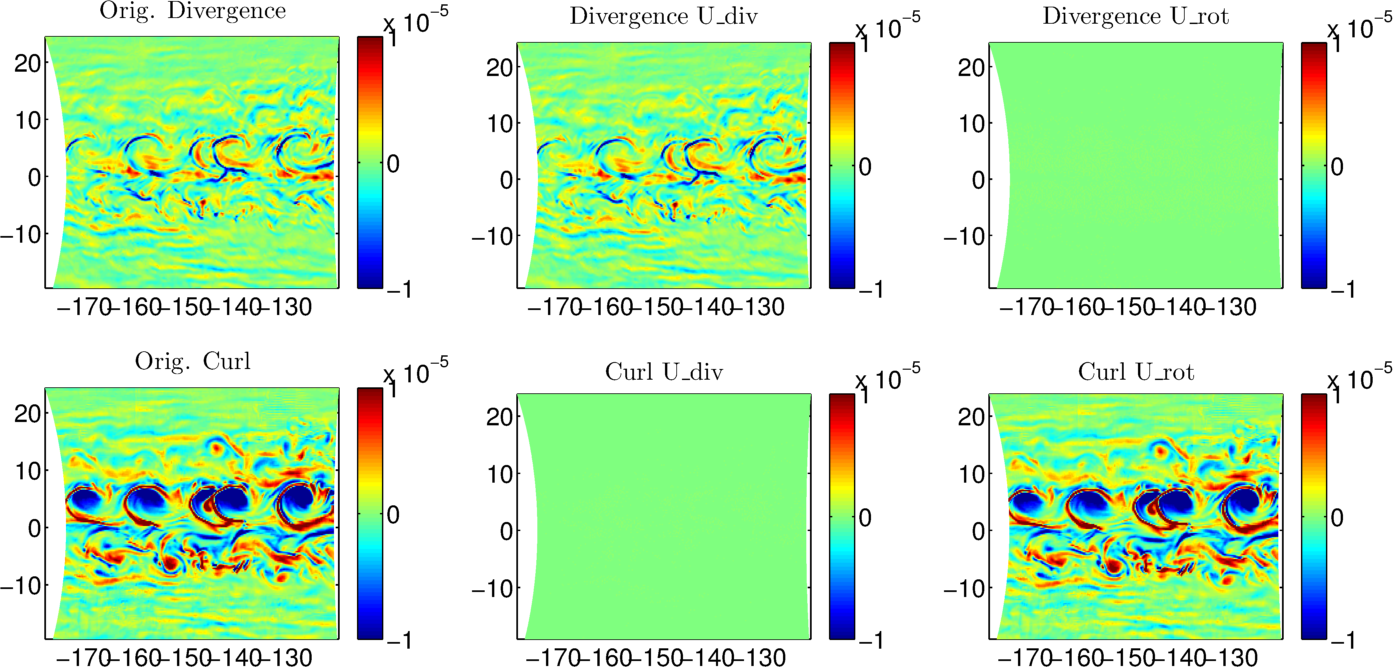
\includegraphics[width=16cm]{CorrectDivCurl.png}
\caption{Figure showing an example calculation where (left) full
  divergence and curl (middle) divergence and curl of $\bm{u}_{div}$ and
(right) divergence and curl of $\bm{u}_{rot}$}
\label{EqSlice}
\end{figure}
\begin{figure}[h!]
\noindent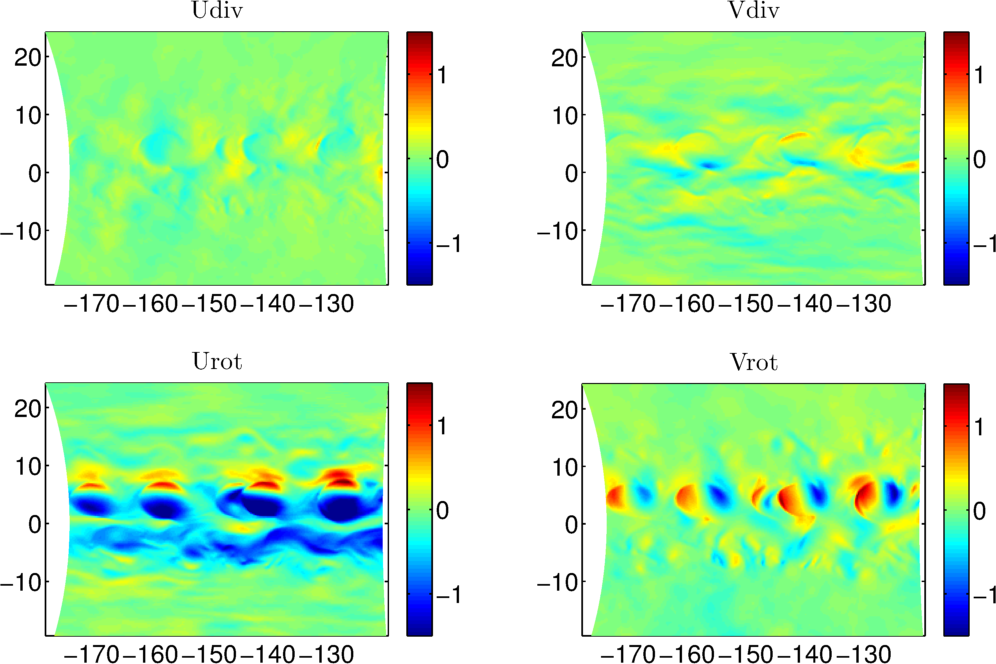
\includegraphics[width=10cm]{CorrectDivRotVel.png}
\caption{Figure showing $\bm{u}_{rot}$ and $\bm{u}_{div}$ for the same
  fields as in Fig. 1}
\label{EqSlice}
\end{figure}
\begin{figure}[h!]
\noindent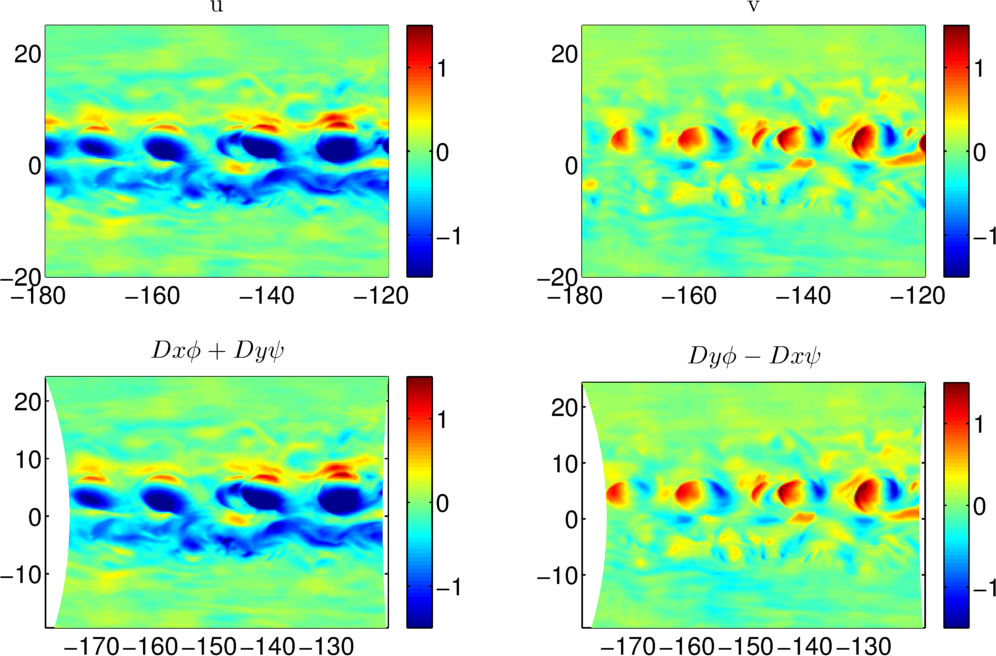
\includegraphics[width=10cm]{CorrectVel.png}
\caption{Figure comparing the full velocities and the velocities
  calculated using the potentials $\phi$ and $\psi$}
\label{EqSlice}
\end{figure}
\begin{figure}[h!]
\noindent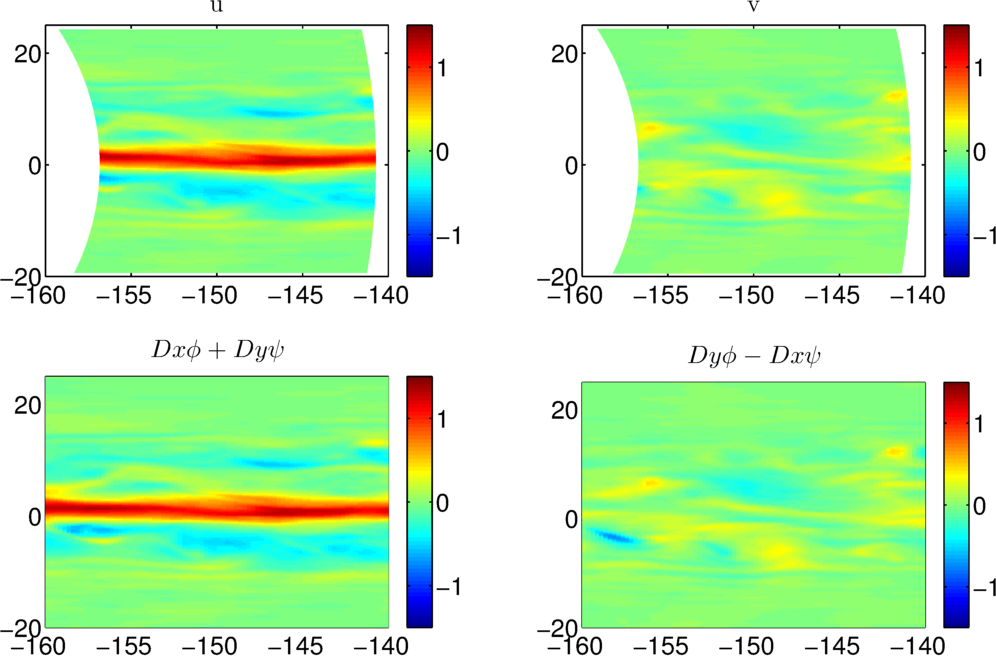
\includegraphics[width=10cm]{DeepCheck1.png}
\caption{Figure comparing the full velocities and the velocities
  calculated using the potentials $\phi$ and $\psi$ for a deeper
  slice.}
\label{EqSlice}
\end{figure}


\end{document}
